\documentclass[11pt,a4paper]{article}
\usepackage[margin=2.3cm]{geometry}
\IfFileExists{lmodern.sty}{\usepackage{lmodern}}{}
\usepackage[T1]{fontenc}
\usepackage{titlesec,tabularx,longtable,booktabs,array,enumitem,xcolor,fancyhdr,amsmath}
\usepackage{listings}
\usepackage{tikz}
\usetikzlibrary{arrows.meta,positioning,fit,calc,shapes.geometric,backgrounds}
\usepackage[hyphens]{url}
\usepackage{hyperref}

\definecolor{headcolor}{RGB}{15,70,60}
\definecolor{boxa}{RGB}{226,239,236}
\definecolor{boxb}{RGB}{238,242,250}
\definecolor{boxc}{RGB}{250,243,230}
\definecolor{boxd}{RGB}{245,245,245}
\definecolor{edge}{RGB}{70,70,70}
\hypersetup{colorlinks=true,linkcolor=headcolor,urlcolor=headcolor,
  pdftitle={TrustBazaar System Design - Unit 2: Order, Payment and Escrow},
  pdfauthor={S. M. Nihal Ahmed, Afrim Hossen Khan, Sabikun Nahar Sinthia}}

\titleformat{\section}{\normalfont\Large\bfseries\color{headcolor}}{\thesection}{10pt}{}
\titleformat{\subsection}{\normalfont\large\bfseries}{\thesubsection}{8pt}{}
\titleformat{\subsubsection}{\normalfont\normalsize\bfseries}{\thesubsubsection}{6pt}{}
\pagestyle{fancy}\fancyhf{}
\fancyhead[L]{System Design Document}\fancyhead[R]{Unit 2: Order, Payment \& Escrow}
\fancyfoot[C]{\thepage}\renewcommand{\headrulewidth}{0.4pt}\setlength{\headheight}{14pt}
\setlength{\emergencystretch}{3em}
\setlength{\parskip}{0.45em}\setlength{\parindent}{0pt}

\lstdefinelanguage{SQLpg}{morekeywords={CREATE,TABLE,TYPE,AS,ENUM,PRIMARY,KEY,REFERENCES,NOT,NULL,DEFAULT,CHECK,UNIQUE,INDEX,ON,WHERE,TRIGGER,BEFORE,INSERT,UPDATE,DELETE,FOR,EACH,ROW,EXECUTE,FUNCTION,RETURNS,LANGUAGE,BEGIN,END,IF,THEN,ELSE,RETURN,SELECT,FROM,INTO,ORDER,BY,DESC,LIMIT,GRANT,REVOKE,TO,SCHEMA,EXTENSION,EXISTS,OR,AND,IN,IS,ALTER,ADD,FOREIGN,GENERATED,ALWAYS,IDENTITY,DEFERRABLE,INITIALLY,DEFERRED,DECLARE,PERFORM,LOOP,RAISE,EXCEPTION,USING,DISTINCT,ROLE,LOGIN,USAGE,ALL,TABLES,STABLE,DO},sensitive=false,morecomment=[l]{--},morestring=[b]'}
\lstset{basicstyle=\ttfamily\scriptsize,columns=fullflexible,keepspaces=true,breaklines=true,
  keywordstyle=\color{headcolor}\bfseries,commentstyle=\color{gray}\itshape,frame=single,rulecolor=\color{gray!40},
  upquote=true,literate={–}{{--}}1}

\newenvironment{dtable}[1]{\small\begin{longtable}{#1}}{\end{longtable}}

\begin{document}
\begin{titlepage}
\centering
\vspace*{1cm}
{\Large Daffodil International University}\\[0.2cm]
{\large Department of Software Engineering}\\[2cm]
\rule{\linewidth}{0.5pt}\\[0.4cm]
{\huge\bfseries System Design Document}\\[0.3cm]
{\LARGE Unit 2: Order, Payment \& Escrow}\\[0.3cm]
{\large TrustBazaar: A Verified Peer-to-Peer Auction and Marketplace Platform for Used Goods}\\[0.2cm]
\rule{\linewidth}{0.5pt}\\[1.6cm]
{\large S. M. Nihal Ahmed (232-35-002)\\[0.1cm] Afrim Hossen Khan (232-35-076)\\[0.1cm] Sabikun Nahar Sinthia (232-35-475)}\\[1.6cm]
\begin{tabular}{|l|>{\raggedright\arraybackslash}p{8cm}|}
\hline
\textbf{Status} & Draft for team review \\ \hline
\textbf{Version} & 0.1, 14 October 2026 \\ \hline
\textbf{Implements} & SRS v2.0 (\texttt{docs/srs.tex}) \\ \hline
\textbf{Depends on} & Unit 1: Identity \& Access (\texttt{01\_identity\_access.pdf}) \\ \hline
\textbf{Database schema} & \texttt{docs/design/sql/02\_orders\_payments.sql}, tested on PostgreSQL (45 checks and a concurrency test, Appendix B) \\ \hline
\end{tabular}
\vfill
\end{titlepage}
\tableofcontents
\newpage
\section{Introduction}

\subsection{Purpose}
This document is the second unit of TrustBazaar's System Design Document. It specifies how the \emph{Order, Payment \& Escrow} unit meets its requirements in SRS v2.0. Every purchase in TrustBazaar, whether at a fixed price, by auction or for a game account, passes through this unit: it creates the order, collects the payment, holds it in escrow, and releases or refunds it according to the rules. It also keeps the ledger that shows where every poisha went. Acceptance criteria 2, 3, 4 and 6 of the SRS (Appendix~A) depend on this unit.

The unit follows the conventions DC-1 to DC-12 of Unit~1 (\texttt{01\_identity\_access.pdf}, Section~2), adds one convention (DC-13, Section~\ref{sec:dc13}), and uses Unit~1's ports for identity checks, step-up authentication, approvals and audit.

\subsection{Scope}
\textbf{In scope:}
\begin{itemize}[nosep]
  \item orders for fixed-price purchases, auction wins and second-chance offers, with checkout holds and payment windows;
  \item the choice of fulfilment method and the fixed delivery fee;
  \item payment collection through bKash, Nagad and Stripe, with confirmation, deduplication and reconciliation;
  \item the escrow state machine and every way money leaves it: release, auto-release, the game-account protection hold, cancellation, deadline refunds and dispute outcomes;
  \item refunds; seller payout accounts and payouts; the double-entry ledger and settlement records;
  \item commission and delivery margin; featured-listing fees and Pro Seller subscriptions; chargebacks.
\end{itemize}

\textbf{Out of scope, owned by later units:}
\begin{itemize}[nosep]
  \item listing stock and its display (Listings; this unit reserves stock through a port);
  \item the auction close, second-chance selection and non-payment strikes (Auction; this unit reports expired payment windows);
  \item courier booking, handover codes and fares (Delivery; this unit receives fulfilment steps and the delivery event);
  \item credential handover and takeover (Game-Account; this unit receives credential delivery and takeover completion);
  \item the dispute process itself (Disputes; this unit freezes escrow and applies outcomes);
  \item the delivery of notifications (Notifications; this unit emits events).
\end{itemize}

\subsection{Requirements covered}
\begin{itemize}[nosep]
  \item \textbf{Functional:} FR-PAY-01 to FR-PAY-21; FR-MON-01 to FR-MON-10. On the order side: FR-FIX-01 to FR-FIX-05, FR-AUC-14 and FR-AUC-15. On the escrow side: FR-DLV-11 to FR-DLV-13, FR-GAM-10, FR-GAM-17, FR-DSP-02, FR-DSP-06, FR-DSP-10 and FR-DSP-11. Also FR-TNS-05 (payout holds), FR-TNS-07 (order limits) and FR-ACC-11 (closure check).
  \item \textbf{Security:} SEC-PAY-01 to SEC-PAY-07; SEC-LOG-01 for money events.
  \item \textbf{Other:} IF-SW-01 to IF-SW-03; IF-UI-04, IF-UI-05, IF-UI-08; NFR-PERF-06, NFR-PERF-08; NFR-REL-02 to NFR-REL-04; NFR-CMP-02, NFR-CMP-03, NFR-CMP-05; DR-03, DR-05, DR-10.
\end{itemize}

% ------------------------------------------------------------------
\section{Unit Overview}

\subsection{Responsibilities}
\begin{enumerate}[nosep]
  \item Create an order only when stock is reserved and the buyer may transact, and fix its price, fees and fee rates at that moment.
  \item Collect payment on the provider's own page, accept it only on a verified server-side confirmation, and accept each payment at most once.
  \item Hold the money in escrow and let it leave only by the transitions of SRS Table~4.8, under the deadlines of the order.
  \item Record every movement in a balanced double-entry ledger, from which the settlement record and the revenue log are derived.
  \item Pay sellers only into verified accounts, after the cooling-off period, unless a fraud hold applies.
  \item Detect and correct anything the providers and the ledger disagree on.
\end{enumerate}

\subsection{Components}

\begin{figure}[!htbp]
\centering
\resizebox{\textwidth}{!}{%
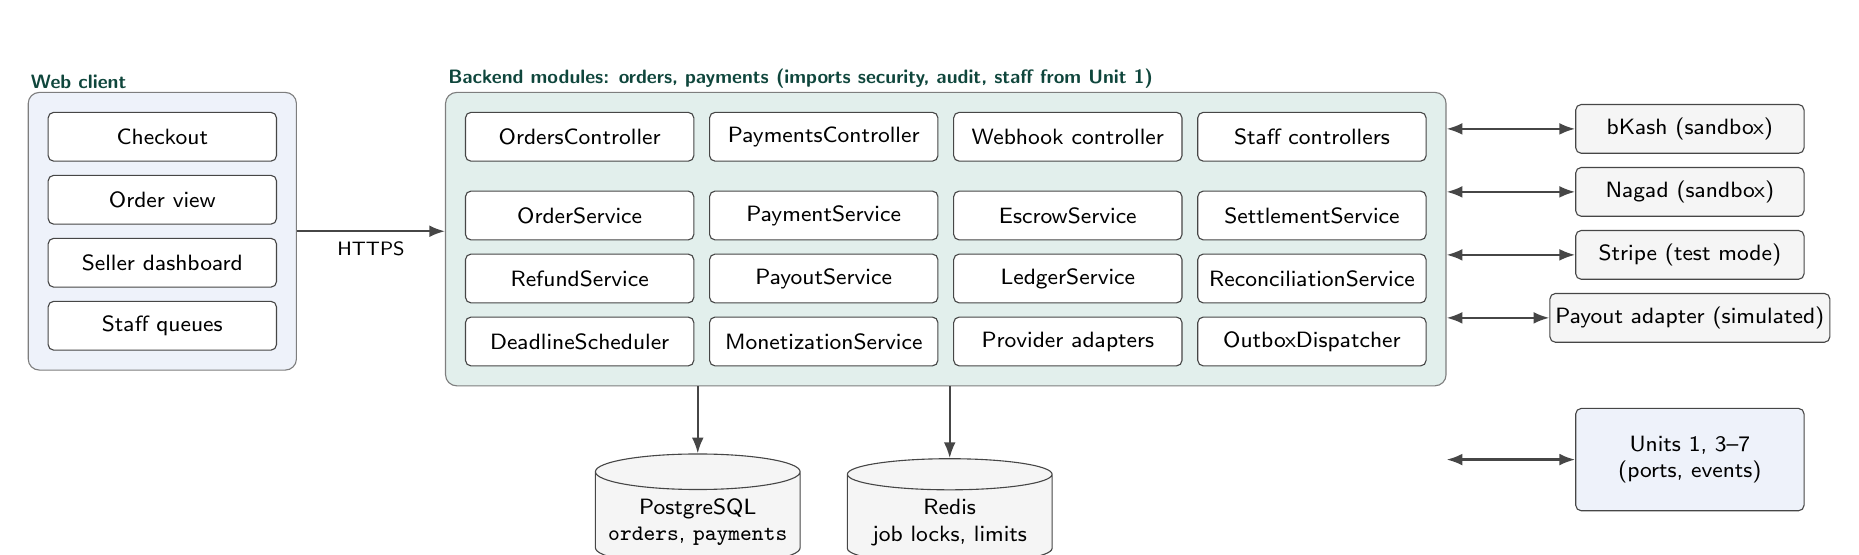
\begin{tikzpicture}[
  font=\sffamily\footnotesize,
  comp/.style={draw=edge, rounded corners=2pt, fill=white, minimum width=2.9cm, minimum height=0.62cm, align=center, inner sep=2pt},
  grp/.style={draw=edge!70, rounded corners=4pt, inner sep=7pt},
  lbl/.style={font=\sffamily\scriptsize\bfseries, text=headcolor, anchor=south west, inner sep=1pt},
  arr/.style={-{Latex[length=2mm]}, draw=edge, thick},
  store/.style={draw=edge, fill=boxd, cylinder, shape border rotate=90, aspect=0.18, minimum width=2.6cm, minimum height=1.1cm, align=center}
]
\node[comp] (c1) at (0,3.9) {Checkout};
\node[comp] (c2) at (0,3.1) {Order view};
\node[comp] (c3) at (0,2.3) {Seller dashboard};
\node[comp] (c4) at (0,1.5) {Staff queues};
\begin{scope}[on background layer]\node[grp, fill=boxb, fit=(c1)(c4)] (client) {};\end{scope}
\node[lbl] at (client.north west) {Web client};

\foreach \n/\x/\y/\t in {k1/5.3/3.9/OrdersController, k2/8.4/3.9/PaymentsController, k3/11.5/3.9/Webhook controller, k4/14.6/3.9/Staff controllers,
  s1/5.3/2.9/OrderService, s2/8.4/2.9/PaymentService, s3/11.5/2.9/EscrowService, s4/14.6/2.9/SettlementService,
  s5/5.3/2.1/RefundService, s6/8.4/2.1/PayoutService, s7/11.5/2.1/LedgerService, s8/14.6/2.1/ReconciliationService,
  s9/5.3/1.3/DeadlineScheduler, s10/8.4/1.3/MonetizationService, s11/11.5/1.3/{Provider adapters}, s12/14.6/1.3/OutboxDispatcher}
  {\node[comp] (\n) at (\x,\y) {\t};}
\begin{scope}[on background layer]\node[grp, fill=boxa, fit=(k1)(k4)(s9)(s12)] (be) {};\end{scope}
\node[lbl] at (be.north west) {Backend modules: orders, payments (imports security, audit, staff from Unit 1)};

\node[store] (pg) at (6.8,-1.0) {PostgreSQL\\\texttt{orders}, \texttt{payments}};
\node[store] (rd) at (10.0,-1.0) {Redis\\job locks, limits};

\node[comp, fill=boxd] (bk) at (19.4,4.0) {bKash (sandbox)};
\node[comp, fill=boxd] (ng) at (19.4,3.2) {Nagad (sandbox)};
\node[comp, fill=boxd] (st) at (19.4,2.4) {Stripe (test mode)};
\node[comp, fill=boxd] (po) at (19.4,1.6) {Payout adapter (simulated)};
\node[comp, fill=boxb, minimum height=1.3cm] (u) at (19.4,-0.2) {Units 1, 3--7\\(ports, events)};

\draw[arr] (client.east) -- node[below, font=\sffamily\scriptsize, align=center]{HTTPS} (be.west|-client.east);
\draw[arr] (pg.north|-be.south) -- (pg.north);
\draw[arr] (rd.north|-be.south) -- (rd.north);
\foreach \t in {bk,ng,st,po}{\draw[arr, {Latex[length=2mm]}-{Latex[length=2mm]}] (be.east|-\t) -- (\t.west);}
\draw[arr, {Latex[length=2mm]}-{Latex[length=2mm]}] (be.east|-u) -- (u.west);
\end{tikzpicture}}
\caption{Components of the Order, Payment \& Escrow unit. Each provider is reached only through its adapter; provider pages are opened in the user's browser by redirect.}
\label{fig:components}
\end{figure}

\begin{dtable}{@{}>{\raggedright\arraybackslash}p{3.6cm}>{\raggedright\arraybackslash}p{11.6cm}@{}}
\toprule
\textbf{Component} & \textbf{Responsibility} \\ \midrule \endhead
OrderService & Creates orders (fixed-price checkout; auction and second-chance orders through the port); sets fulfilment and the delivery fee; enforces order limits; cancels unpaid orders. \\
PaymentService & Starts payment attempts; confirms them from verified provider evidence; handles duplicate, late and mismatched payments. \\
Webhook controller (ProviderEventsController) & Receives Stripe webhooks and bKash and Nagad browser callbacks; verifies them (signature, or verification query) and records each event once. \\
EscrowService & The only component that changes escrow state; applies fulfilment steps, delivery events, buyer releases, cancellations, deadline refunds and dispute outcomes. \\
SettlementService & Computes the split, writes the settlement record and posts the ledger entries on every terminal transition. \\
LedgerService & Posts balanced journal entries; provides balances and the revenue log. \\
RefundService, PayoutService & Execute refunds and payouts through adapters, with idempotency keys, retries and manual fallback. \\
ReconciliationService & Compares in-flight attempts, refunds and payouts with the providers, and raises discrepancies for operators. \\
DeadlineScheduler & Runs the scheduled actions of Section~\ref{sec:jobs}. \\
MonetizationService & Featured-listing purchases and Pro Seller subscriptions; answers ``is this seller Pro?''. \\
Provider adapters & One per provider, behind one interface (Section~\ref{sec:adapters}); a simulated payout adapter. \\
\bottomrule
\end{dtable}

\subsection{New convention: transactional ports}
\label{sec:dc13}
\textbf{DC-13.} A port may take the caller's transaction (\texttt{EntityManager}) as an argument when two units must change state atomically. The callee still writes only its own tables. This unit uses the rule in exactly three places:
\begin{itemize}[nosep]
  \item reserving stock while creating an order (\texttt{ListingsPort.reserve}, FR-FIX-02);
  \item recording a fulfilment step or delivery event reported by Delivery or Game-Account;
  \item applying a dispute outcome decided in Disputes.
\end{itemize}
Every other interaction between units goes through events. To avoid deadlocks, every transaction that locks more than one row locks them in a fixed order: listing, then order, then escrow, then attempt.
\section{Interfaces}

\subsection{HTTP API}
\label{sec:api}
All paths are under \texttt{/api/v1}; policies and rate limits are those of Unit~1 (Section~4.1). Amounts in requests are never trusted (SEC-PAY-06): every price, fee and total is computed on the server from the listing, the delivery quote and the order.

{\small
\begin{longtable}{@{}>{\ttfamily\raggedright\arraybackslash}p{1.15cm}>{\ttfamily\raggedright\arraybackslash}p{4.9cm}>{\raggedright\arraybackslash}p{2.7cm}>{\raggedright\arraybackslash}p{6.2cm}@{}}
\toprule
\textnormal{\textbf{Method}} & \textnormal{\textbf{Path}} & \textbf{Policy} & \textbf{Purpose (requirement)} \\ \midrule \endhead
\multicolumn{4}{@{}l}{\textbf{Buyer}} \\
POST & /\allowbreak orders & Verified(buy) & Fixed-price checkout: reserve stock, create order (FR-FIX-01, 02, 05) \\
GET & /\allowbreak orders?role=buyer|seller & SignedIn & My orders \\
GET & /\allowbreak orders/\allowbreak \{id\} & Party to order & Order, escrow state, deadlines (IF-UI-05) \\
PUT & /\allowbreak orders/\allowbreak \{id\}/\allowbreak fulfilment & Buyer & Choose method and delivery quote (FR-DLV-02, 09) \\
POST & /\allowbreak orders/\allowbreak \{id\}/\allowbreak payments & Verified(buy), buyer & Start payment; returns provider redirect (FR-PAY-01) \\
GET & /\allowbreak payments/\allowbreak return/\allowbreak \{provider\} & Public & Landing page after the provider; shows status only, never confirms (FR-PAY-02) \\
POST & /\allowbreak orders/\allowbreak \{id\}/\allowbreak confirm-\allowbreak receipt & Buyer & Release after the delivery event (FR-PAY-07a) \\
POST & /\allowbreak orders/\allowbreak \{id\}/\allowbreak release-\allowbreak early & Buyer, StepUp & Game account: release before the protection period ends (FR-GAM-17) \\
POST & /\allowbreak orders/\allowbreak \{id\}/\allowbreak cancellation-\allowbreak requests & Buyer & Ask to cancel before the delivery event (FR-PAY-09) \\
GET & /\allowbreak orders/\allowbreak \{id\}/\allowbreak receipt & Party to order & Receipt or statement (FR-PAY-21) \\
\multicolumn{4}{@{}l}{\textbf{Seller}} \\
POST & /\allowbreak orders/\allowbreak \{id\}/\allowbreak cancellation-\allowbreak requests/\allowbreak \{rid\}/\allowbreak decision & Seller & Accept or decline (FR-PAY-09) \\
POST & /\allowbreak orders/\allowbreak \{id\}/\allowbreak cancel & Seller & Cancel after payment, before delivery; refund and strike (FR-PAY-09) \\
GET & /\allowbreak me/\allowbreak payout-\allowbreak account & Verified & Current account and status \\
POST & /\allowbreak me/\allowbreak payout-\allowbreak account & Verified(payout), StepUp & Add or replace (FR-PAY-17, 18) \\
GET & /\allowbreak me/\allowbreak payouts, /\allowbreak me/\allowbreak statements & Verified & Payout history, settlement statements \\
POST & /\allowbreak listings/\allowbreak \{id\}/\allowbreak feature & Verified(list), seller & Buy featured placement (FR-MON-05) \\
POST, DELETE & /\allowbreak me/\allowbreak subscription & Verified & Start or cancel Pro Seller (FR-MON-06, 08) \\
\multicolumn{4}{@{}l}{\textbf{Providers} (no session; verified per Section~\ref{sec:verify})} \\
POST & /\allowbreak webhooks/\allowbreak stripe & Stripe signature & Checkout, refund, dispute events \\
GET & /\allowbreak callbacks/\allowbreak bkash/\allowbreak \{attemptId\} & Signed state & bKash browser callback; triggers Execute and Query \\
GET & /\allowbreak callbacks/\allowbreak nagad/\allowbreak \{attemptId\} & Signed state & Nagad browser callback; triggers Verify \\
\multicolumn{4}{@{}l}{\textbf{Staff}} \\
GET & /\allowbreak staff/\allowbreak payments/\allowbreak issues & Staff(operator) & Reconciliation queue (FR-OPS-01) \\
POST & /\allowbreak staff/\allowbreak payments/\allowbreak issues/\allowbreak \{id\}/\allowbreak resolve & Staff(operator) & Resolve with a recorded reason \\
GET & /\allowbreak staff/\allowbreak payout-\allowbreak accounts/\allowbreak pending & Staff(operator) & Bank accounts awaiting the name check \\
POST & /\allowbreak staff/\allowbreak payout-\allowbreak accounts/\allowbreak \{id\}/\allowbreak decision & Staff(operator) & Approve or reject (FR-PAY-17) \\
POST & /\allowbreak staff/\allowbreak payouts/\allowbreak \{id\}/\allowbreak release-\allowbreak hold & Staff(operator) & Lift a fraud hold (FR-TNS-05) \\
\bottomrule
\end{longtable}
}

\subsection{Provider adapters}
\label{sec:adapters}
Each provider is wrapped in an adapter implementing one interface, so the rest of the unit never sees a provider's own API. The exact endpoints, field names and signing schemes follow each provider's documentation [SRS R13] and are confined to the adapter.
\begin{lstlisting}[language=Java,morekeywords={interface,type,Promise,string,boolean,number,bigint}]
interface PaymentProvider {
  readonly id: 'bkash' | 'nagad' | 'stripe';
  createPayment(a: { attemptId: string; amount: bigint; idempotencyKey: string;
      returnUrl: string }): Promise<{ providerPaymentId: string; redirectUrl: string }>;
  // turns provider evidence into a verified result; never trusts the browser
  verify(input: CallbackInput | WebhookInput): Promise<VerifiedResult>;
  query(attempt: Attempt): Promise<VerifiedResult>;        // reconciliation and expiry checks
  refund(r: { attempt: Attempt; amount: bigint; idempotencyKey: string }):
      Promise<{ status: 'succeeded' | 'pending' | 'unsupported'; providerRefundId?: string }>;
}
type VerifiedResult = { eventId: string; providerPaymentId: string; providerTxnId?: string;
  status: 'succeeded' | 'failed' | 'pending'; amount: bigint; currency: string;
  merchantReference: string /* = attemptId */; verifiedBy: 'signature' | 'query' };
interface PayoutProvider { send(p: { payoutId: string; amount: bigint; destination: PayoutAccount;
  idempotencyKey: string }): Promise<{ status: 'sent' | 'failed'; ref?: string }>; }
\end{lstlisting}

\begin{dtable}{@{}>{\bfseries}p{1.6cm}>{\raggedright\arraybackslash}p{13.6cm}@{}}
\toprule
\textnormal{\textbf{Provider}} & \textbf{How a payment is made and confirmed} \\ \midrule \endhead
bKash & Tokenized Checkout. The adapter obtains a grant token and creates a payment, passing the attempt id as the merchant invoice number. The buyer enters wallet number, OTP and PIN on bKash's page. bKash redirects the browser to our callback, carrying the payment id and a status. \emph{The callback status is not trusted.} The server calls Execute Payment, and Query Payment if the outcome is unclear, and accepts only a completed transaction whose amount, currency and invoice number match. Refunds use bKash's refund function with the payment id, transaction id and amount; partial refunds are supported. \\
Nagad & Merchant checkout. The adapter initialises and completes a checkout with the attempt id as the order id; the buyer pays on Nagad's page. The callback carries a payment reference, which the server verifies with Nagad's verification API before accepting. If the sandbox offers no refund function, a refund is marked \texttt{manual\_required} and placed in the operator queue (FR-PAY-12). \\
Stripe & Stripe Checkout, the hosted payment page, reached by redirect, in test mode. The attempt id is sent as the client reference, and the attempt's idempotency key on every API call. Confirmation comes from the \texttt{checkout.session.completed} webhook, verified with the \texttt{Stripe-Signature} header within the CP-32 tolerance. Refunds use the refunds API with an idempotency key. \texttt{charge.dispute.created} records a chargeback (FR-PAY-20). Because the card form is entirely on Stripe's page and is reached by redirect, the merchant is eligible for SAQ A without the script-protection criterion that applies to embedded forms [SRS R6]. \\
Payouts & No disbursement sandbox is assumed (SRS OI-4). The simulated adapter records a reference and marks payouts \texttt{simulated}; a real adapter replaces it without other changes. \\
\bottomrule
\end{dtable}

\subsection{Ports provided to other units}
\begin{lstlisting}[language=Java,morekeywords={interface,type,Promise,string,boolean,number,bigint}]
interface OrdersPort {                                   // used by the Auction unit
  createAuctionOrder(a: { listingId: string; winnerId: string; price: bigint;
      kind: 'auction' | 'second_chance' }): Promise<Order>;   // payment window CP-10 / CP-11
  getOrderForParty(orderId: string, userId: string): Promise<OrderView>;
}
interface EscrowCommands {                               // used by Delivery, Game-Account, Disputes
  recordFulfilmentStep(orderId: string, step: FulfilmentStep, at: Date, tx: EntityManager): Promise<void>;
  recordDeliveryEvent(orderId: string, source: DeliverySource, at: Date, tx: EntityManager): Promise<void>;
  refundCourierReturned(orderId: string, courierCharge: bigint, tx: EntityManager): Promise<void>;
  freezeForDispute(orderId: string, disputeId: string, tx: EntityManager): Promise<void>;
  applyDisputeOutcome(orderId: string, disputeId: string, o: DisputeOutcome,
      tx: EntityManager): Promise<void>;                 // release | full | partial(itemRefund)
  withdrawDispute(orderId: string, disputeId: string, tx: EntityManager): Promise<void>;
}
interface EscrowQuery {
  getEscrow(orderId: string): Promise<EscrowView>;         // state, deadlines, amounts
  disputeAllowed(orderId: string, at: Date): Promise<boolean>;   // held and inside the window
}
interface ProStatusQuery { isPro(userId: string): Promise<boolean> }   // Listings: limit CP-28
// Unit 1's AccountClosureCheck is implemented here: open orders, unpaid wins, balance owed.
\end{lstlisting}

\subsection{Events published}
All are written to \texttt{orders.outbox} in the same transaction as the change (DC-6).
\begin{dtable}{@{}>{\ttfamily}p{6.0cm}>{\raggedright\arraybackslash}p{9.2cm}@{}}
\toprule
\textnormal{\textbf{Event}} & \textbf{Consumers and purpose} \\ \midrule \endhead
orders.order.created & Notifications. \\
orders.order.paid & Listings: mark units sold (FR-FIX-04). Delivery: book the courier or open the meetup flow. Game-Account: ask the seller for credentials (FR-GAM-10). Notifications. \\
orders.order.cancelled & Listings: return reserved stock (FR-FIX-03). Notifications. \\
orders.order.\allowbreak payment\_expired & Auction: second-chance offer and non-payment strike (FR-AUC-15, FR-AUC-16). \\
orders.order.delivered & Notifications: dispute window and release date (FR-NTF-07). \\
orders.escrow.frozen & Notifications. \\
orders.escrow.\allowbreak released, .refunded, .partially\_refunded & Reviews: rating unlocked (FR-REV-01). Notifications. \\
orders.order.\allowbreak cancelled\_by\_seller & Trust \& Safety: seller strike (FR-PAY-09, FR-TNS-04). \\
payments.refund.\allowbreak manual\_required, payments.payout.\allowbreak failed & Notifications; operator queue. \\
payments.payout\_account.changed & Notifications: alert to the seller's number and e-mail (FR-PAY-18). \\
payments.featured.\allowbreak started, .ended; payments.\allowbreak subscription.\allowbreak changed & Listings: featured label, listing limit (FR-MON-05, FR-MON-08). \\
\bottomrule
\end{dtable}

\subsection{Ports required}
\begin{dtable}{@{}>{\ttfamily}p{4.4cm}>{\raggedright\arraybackslash}p{10.8cm}@{}}
\toprule
\textnormal{\textbf{Port}} & \textbf{Provider and use} \\ \midrule \endhead
IdentityQuery (Unit 1) & \texttt{assertCanTransact}; \texttt{getVerifiedPhone} for MFS payout accounts; \texttt{getKycLegalName} for the bank-account check; the date of verification for CP-27 (an addition to the Unit~1 port, noted in Section~\ref{sec:notes}). \\
StepUpGuard, ApprovalService, AuditService (Unit 1) & Step-up for payout changes and early release; audit of every money action. \\
ListingsPort (Unit 3) & \texttt{reserve(listingId, qty, tx)} and \texttt{release(listingId, qty, tx)}: one conditional update each (DC-13); \texttt{snapshot(listingId)} for the order. \\
DeliveryPort (Unit 4) & \texttt{getQuote(quoteId)}: fee, expiry, buyer and listing it was issued for. \\
GameAccountPort (Unit 5) & \texttt{assertCheckoutReady(orderId)}: disclosure acknowledged and buyer public key present (FR-GAM-05, FR-GAM-07). \\
ConfigPort & CP values; their version is stored on each order. \\
\bottomrule
\end{dtable}
\section{Data Design}
\label{sec:data}
The schema is in \texttt{docs/design/sql/02\_orders\_payments.sql} (Appendix~\ref{app:ddl}). It is loaded after Unit~1's schema and references only \texttt{identity.users} and \texttt{identity.staff\_accounts} (DC-5). The unit owns two schemas: \texttt{orders} (orders, escrow and its history, cancellation requests, outbox) and \texttt{payments} (attempts, provider events, refunds, payout accounts, payouts, ledger, settlements, reconciliation issues and monetization).

\tikzset{
  ent/.style={draw=edge, fill=white, rounded corners=1.5pt, align=left, inner sep=3pt, font=\sffamily\scriptsize, text width=3.75cm},
  fk/.style={-{Latex[length=1.6mm]}, draw=edge!80, semithick},
}
\newcommand{\ent}[2]{\textbf{\color{headcolor}#1}\\[-1pt]{\ttfamily\tiny #2}}

\begin{figure}[!htbp]
\centering
\resizebox{0.98\textwidth}{!}{%
\begin{tikzpicture}
\node[ent, fill=boxd] (users) at (0,5.6) {\ent{identity.users}{(Unit 1)}};
\node[ent, fill=boxa, text width=4.6cm] (ord) at (5.6,4.2) {\ent{orders.orders}{id PK, kind, listing\_id (Unit 3)\\buyer\_id $\neq$ seller\_id\\quantity, unit\_price, item\_price\\fulfilment, delivery\_quote\_id\\delivery\_fee, total\\listing\_snapshot, commission\_bps,\\delivery\_margin\_bps, params\_version\\status, payment\_due\_at, paid\_at\\fulfilment\_step / due / done\\delivery\_event\_at / source\\cancelled\_at, closed\_at}};
\node[ent, fill=boxc] (esc) at (11.4,5.3) {\ent{orders.escrows}{order\_id PK\\state (trigger-checked)\\release\_policy\\amount\_collected / released / refunded\\dispute\_window\_ends\_at\\auto\_release\_at\\open\_dispute\_id (Unit 7)}};
\node[ent] (hist) at (11.4,2.2) {\ent{orders.escrow\_history}{append-only\\from / to state, actor\\reason, amounts, related\_id}};
\node[ent] (canc) at (0,2.6) {\ent{orders.cancellation\_requests}{one pending per order\\requested\_by, reason, status}};
\node[ent, fill=boxd] (ob) at (0,0.6) {\ent{orders.outbox}{event\_type, payload\\dispatched\_at}};
\draw[fk] (ord.north west) -- ++(0,0.5) -| ([xshift=10pt]users.south) node[pos=0.2, above, font=\sffamily\tiny]{buyer\_id, seller\_id};
\draw[fk] (esc.west) -- (ord.east|-esc.west);
\draw[fk] (hist.west) -- (ord.east|-hist.west);
\draw[fk] (canc.east) -- (ord.west|-canc.east);
\end{tikzpicture}}
\caption{Orders and escrow (schema \texttt{orders}). Each paid order has exactly one escrow row, whose state can change only along the edges of Figure~\ref{fig:states}.}
\label{fig:er-orders}
\end{figure}

\begin{figure}[!htbp]
\centering
\resizebox{0.98\textwidth}{!}{%
\begin{tikzpicture}
\node[ent, fill=boxd] (ord) at (0,6.2) {\ent{orders.orders}{(Figure~\ref{fig:er-orders})}};
\node[ent, fill=boxa] (att) at (5.2,6.2) {\ent{attempts}{id PK (= merchant reference)\\purpose, order\_id, payer\_id\\provider, amount, BDT only\\idempotency\_key UNIQUE\\provider\_payment\_id, txn\_id\\status; one success per order}};
\node[ent] (ev) at (10.4,6.2) {\ent{provider events}{UNIQUE (provider, event\_id)\\verified\_by, payload\_sha256\\attempt\_id, processed\_at}};
\node[ent] (ref) at (5.2,3.1) {\ent{refunds}{attempt\_id, order\_id, amount\\reason, idempotency\_key\\status; total $\le$ payment}};
\node[ent] (cb) at (10.4,3.6) {\ent{chargebacks}{attempt\_id, provider\_case\_id\\amount, recovered}};
\node[ent] (pa) at (0,1.0) {\ent{payout accounts}{user\_id, kind (wallet / bank)\\wallet\_e164 or bank fields\\account\_number\_enc\\status, effective\_at\\one current per seller}};
\node[ent] (po) at (5.2,0.4) {\ent{payouts}{order\_id UNIQUE, seller\_id\\payout\_account\_id, amount\\status, hold\_reason, simulated\\idempotency\_key}};
\node[ent, fill=boxc] (je) at (10.4,1.1) {\ent{journal entries and lines}{entry: kind, order\_id, source\_id\\line: account\_code, party\_id,\\amount (debit + / credit $-$)\\each entry sums to zero\\append-only}};
\node[ent] (st) at (15.4,6.2) {\ent{settlements}{order\_id PK\\collected, item, fee\\commission, courier, margin\\seller\_payout, refund\_total\\parts = collected}};
\node[ent] (la) at (15.4,1.6) {\ent{ledger accounts}{code PK, kind\\12 fixed accounts}};
\node[ent] (rec) at (15.4,3.9) {\ent{reconciliation issues}{kind, links, detail\\status, resolved\_by}};
\node[ent] (mon) at (0,3.9) {\ent{featured purchases,\\subscriptions}{Could Have\\paid through attempts}};
\draw[fk] (att.west) -- (ord.east);
\draw[fk] (ev.west) -- (att.east);
\draw[fk] (ref.north) -- (att.south);
\draw[fk] (cb.north west) -- ([yshift=-8pt]att.east);
\draw[fk] (po.west) -- (pa.east|-po.west);
\draw[fk] (je.east) -- (la.west|-je.east);
\draw[fk] (mon.north east) -- ([yshift=-8pt]att.west);
\end{tikzpicture}}
\caption{Payments, payouts and the ledger (schema \texttt{payments}). Settlements, refunds, payouts and journal entries also reference \texttt{orders.orders}; those arrows are omitted for legibility.}
\label{fig:er-payments}
\end{figure}

\subsection{Tables}
\begin{dtable}{@{}>{\ttfamily\raggedright\arraybackslash}p{3.7cm}>{\raggedright\arraybackslash}p{4.9cm}>{\raggedright\arraybackslash}p{6.6cm}@{}}
\toprule
\textnormal{\textbf{Table}} & \textbf{Holds} & \textbf{Rules enforced by the database} \\ \midrule \endhead
orders.\allowbreak orders & One row per order with a snapshot of the listing and the fee rates in force (DR-03, FR-MON-10). & Buyer is not the seller; item price $=$ unit price $\times$ quantity; total $=$ item price $+$ fee; auctions have quantity 1; a fee only for courier, and courier only with a quote; game accounts only by game-account handover; no payment before a fulfilment method; a paid order has a fulfilment deadline; a delivery event only after the fulfilment step; at most one live order per auction listing. \\
orders.\allowbreak escrows & One row per paid order. & Starts in \texttt{held}; only the transitions of SRS Table~4.8 (trigger); amounts consistent with the state (nothing paid out while open; released $+$ refunded $=$ collected when terminal; a partial refund has both); a frozen escrow names its dispute; the dispute window ends no later than auto-release; terminal rows never change; the collected amount never changes. \\
orders.\allowbreak escrow\_history & Every transition with actor, reason and amounts (FR-PAY-10). & Append-only (trigger and grants). \\
orders.\allowbreak cancellation\_requests & Buyer requests before the delivery event. & One pending request per order. \\
payments.\allowbreak attempts & Each attempt to pay, with its idempotency key and provider references. & BDT only; \textbf{one successful attempt per order} (acceptance criterion 4); provider references unique. \\
payments.\allowbreak provider\_events & Every verified webhook, callback or query result. & \textbf{Unique per provider and event id}, so a replay has no effect (SEC-PAY-04). \\
payments.\allowbreak refunds & Each refund, linked to the original payment. & The total refunded from a payment can never exceed it (trigger). \\
payments.\allowbreak payout\_accounts & Wallet or bank details (account number encrypted). & One current account per seller; a bank account is usable only after an operator's name check; a usable account has a cooling-off end time. \\
payments.\allowbreak payouts & One payout per order. & One per order; an account is required unless the payout is waiting for one or held; a hold records its reason. \\
payments.\allowbreak journal\_entries / \_lines & The double-entry ledger. & Every entry balances (deferred constraint trigger, checked at commit); append-only. \\
payments.\allowbreak settlements & The settlement record of FR-PAY-13. & Parts add up exactly to the amount collected; courier payout $+$ margin $\le$ delivery fee; append-only. \\
payments.\allowbreak ledger\_accounts & The chart of accounts. & Not changeable by the application role. \\
\bottomrule
\end{dtable}

\subsection{The guarantees, and why they live in the database}
\begin{enumerate}[nosep]
  \item \textbf{An order is paid only once} (AC-4). The confirmation path is idempotent in code, and the database adds two independent barriers. A provider event can be recorded only once, and an order can have only one \texttt{succeeded} attempt. A second payment that really succeeded at the provider, for example from two browser tabs, is stored as \texttt{succeeded\_duplicate} and refunded in full. The concurrency test of Appendix~\ref{app:tests} sends 15 confirmations at once, 10 copies of one webhook and 5 different confirmations; exactly one escrow results.
  \item \textbf{Money leaves escrow only by permitted transitions} (AC-3, AC-6). The trigger \texttt{escrow\_transition} rejects any other change and any change to a terminal escrow, whatever the application does.
  \item \textbf{Every poisha is accounted for} (FR-PAY-14). Every journal entry must sum to zero when its transaction commits, and every settlement record must add up to the amount collected. A refund can never exceed its payment.
  \item \textbf{History cannot be rewritten.} Escrow history, journal entries and lines, and settlements are append-only by trigger, and the application role has no \texttt{UPDATE} on them.
\end{enumerate}

\subsection{The ledger}
\label{sec:ledger}
Debits are positive and credits negative, so each entry sums to zero. \texttt{party\_id} identifies the order, seller or buyer a line belongs to. Table~\ref{tab:postings} lists the entries the unit posts; every money event in the system is one of them.

\begin{table}[!htbp]
\centering
\small
\caption{Journal entries posted by the unit (Dr = debit, Cr = credit).}
\label{tab:postings}
\begin{tabularx}{\textwidth}{@{}>{\raggedright\arraybackslash}p{3.2cm} X@{}}
\toprule
\textbf{Event} & \textbf{Entry} \\ \midrule
Payment confirmed & Dr provider\_clearing (total) / Cr escrow\_liability [order] (total). \\
Release & Dr escrow\_liability (total) / Cr seller\_payable [seller], revenue\_commission, courier\_payable, revenue\_delivery\_margin. \\
Full refund & Dr escrow\_liability (total) / Cr buyer\_refund\_payable [buyer]. \\
Partial refund & Dr escrow\_liability (total) / Cr buyer\_refund\_payable, seller\_payable, revenue\_commission, and courier\_payable with revenue\_delivery\_margin if the courier picked up. \\
Refund paid out & Dr buyer\_refund\_payable / Cr provider\_clearing. \\
Duplicate, late or mismatched payment & Dr provider\_clearing / Cr buyer\_refund\_payable (money in, owed straight back). \\
Payout sent & Dr seller\_payable / Cr payout\_clearing. \\
Courier settled & Dr courier\_payable / Cr payout\_clearing. \\
Courier return charge & Dr expense\_courier\_returns / Cr courier\_payable (FR-DLV-12). \\
Featured fee, subscription & Dr provider\_clearing / Cr revenue\_featured or revenue\_subscription. \\
Chargeback & Dr seller\_receivable [seller] / Cr provider\_clearing; recovered later by Dr seller\_payable / Cr seller\_receivable. \\
\bottomrule
\end{tabularx}
\end{table}

The settlement record of an order is derived from the same numbers as its release or refund entry and is written in the same transaction. The revenue log (FR-MON-09) is the view \texttt{payments.revenue\_log}: every line on a \texttt{revenue\_*} account. It is separate from the settlement records, as the SRS requires. In production the \texttt{provider\_clearing} and \texttt{escrow\_liability} balances correspond to funds held by the Bangladesh Bank-licensed provider (SRS C-7); the platform instructs movements but does not hold the money itself.

\subsection{The split}
\label{sec:split}
\texttt{payments.split(item\_price, delivery\_fee, item\_refund, courier\_done, commission\_bps, margin\_bps)} is the reference implementation of SRS FR-PAY-11, FR-PAY-14, FR-MON-01 and FR-DLV-13. The application's \texttt{SettlementService} implements the same rules, and a test compares the two on random inputs.
\begin{enumerate}[nosep]
  \item A refund is taken from the item price first: \textit{released} $=$ item price $-$ item refund.
  \item Commission $=$ $\lfloor(\textit{released} \times \textit{commission\_bps} + 5000)/10000\rfloor$, which is half-up rounding to the poisha.
  \item If the courier picked the item up, the delivery fee is earned. The margin is computed in the same way, and the courier payout $=$ fee $-$ margin. Otherwise the whole fee is refunded.
  \item Seller payout $=$ \textit{released} $-$ commission, calculated last as the remainder.
\end{enumerate}
The parts therefore always sum to item price $+$ fee. The test script checks this on the SRS worked example (BDT 500 $+$ 15 $+$ 135 $+$ 9{,}500 $=$ 10{,}150) and on its partial-refund variant. It also checks 20{,}000 random cases, which all add up exactly with no negative part.

An early draft of the function took the refund as a single amount and could leave part of an unused delivery fee unallocated. Restating it in terms of the \emph{item} refund, with the fee rule applied separately, removed that case.
\section{Behaviour}

\subsection{Order and escrow states}
\begin{figure}[!htbp]
\centering
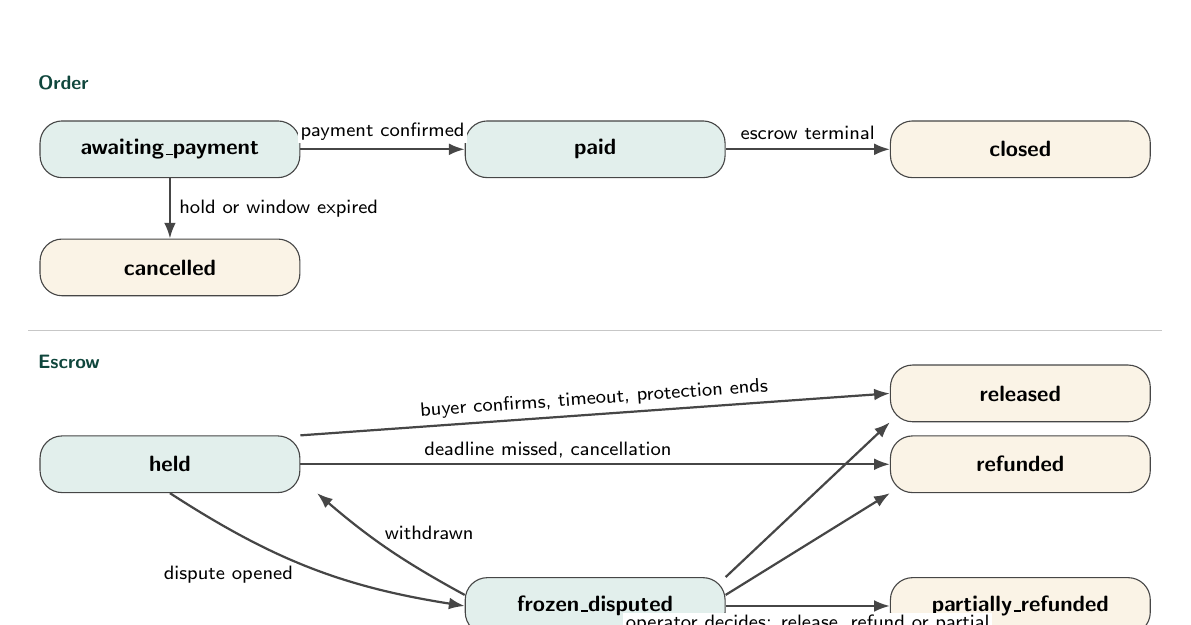
\begin{tikzpicture}[font=\sffamily\footnotesize,
  st/.style={draw=edge, rounded corners=8pt, fill=boxa, minimum width=3.3cm, minimum height=0.72cm, font=\sffamily\footnotesize\bfseries},
  tst/.style={st, fill=boxc},
  tr/.style={-{Latex[length=2mm]}, draw=edge, thick},
  lb/.style={font=\sffamily\scriptsize, align=center, fill=white, inner sep=1pt}]
\node[font=\sffamily\scriptsize\bfseries, text=headcolor, anchor=west] at (-1.8,1.25) {Order};
\node[st] (aw) at (0,0.4) {awaiting\_payment};
\node[st] (pd) at (5.4,0.4) {paid};
\node[tst] (cl) at (10.8,0.4) {closed};
\node[tst] (cn) at (0,-1.1) {cancelled};
\draw[tr] (aw) -- node[lb, above=2pt]{payment confirmed} (pd);
\draw[tr] (pd) -- node[lb, above=2pt]{escrow terminal} (cl);
\draw[tr] (aw) -- node[lb, right=2pt]{hold or window expired} (cn);
\draw[draw=edge!30] (-1.8,-1.9) -- (12.6,-1.9);
\node[font=\sffamily\scriptsize\bfseries, text=headcolor, anchor=west] at (-1.8,-2.3) {Escrow};
\node[st] (h) at (0,-3.6) {held};
\node[st] (f) at (5.4,-5.4) {frozen\_disputed};
\node[tst] (r) at (10.8,-2.7) {released};
\node[tst] (rf) at (10.8,-3.6) {refunded};
\node[tst] (pr) at (10.8,-5.4) {partially\_refunded};
\draw[tr] (h.north east) -- node[lb, sloped, above=1pt]{buyer confirms, timeout, protection ends} (r.west);
\draw[tr] (h.east) -- node[lb, above=1pt, pos=0.42]{deadline missed, cancellation} (rf.west);
\draw[tr] (h.south) to[bend right=12] node[lb, below left=0pt, pos=0.45]{dispute opened} (f.west);
\draw[tr] ([yshift=4pt]f.west) to[bend left=6] node[lb, above right=0pt, pos=0.55]{withdrawn} ([xshift=6pt]h.south east);
\draw[tr] (f.north east) -- (r.south west);
\draw[tr] (f.east) ++(0,4pt) -- (rf.south west);
\draw[tr] (f.east) -- node[lb, below=2pt, pos=0.5]{operator decides: release, refund or partial} (pr.west);
\end{tikzpicture}
\caption{Order status (top) and escrow state (bottom). Terminal states are shaded. The escrow edges are exactly those of SRS Table~4.8, and the database trigger refuses any other.}
\label{fig:states}
\end{figure}

\subsection{Deadlines}
\label{sec:deadlines}
Every order carries the deadlines that apply to it as columns, so a scheduled job can find due work with an index scan and act on recorded times (NFR-REL-03). Figure~\ref{fig:timeline} shows them in order.

\begin{figure}[!htbp]
\centering
\resizebox{\textwidth}{!}{%
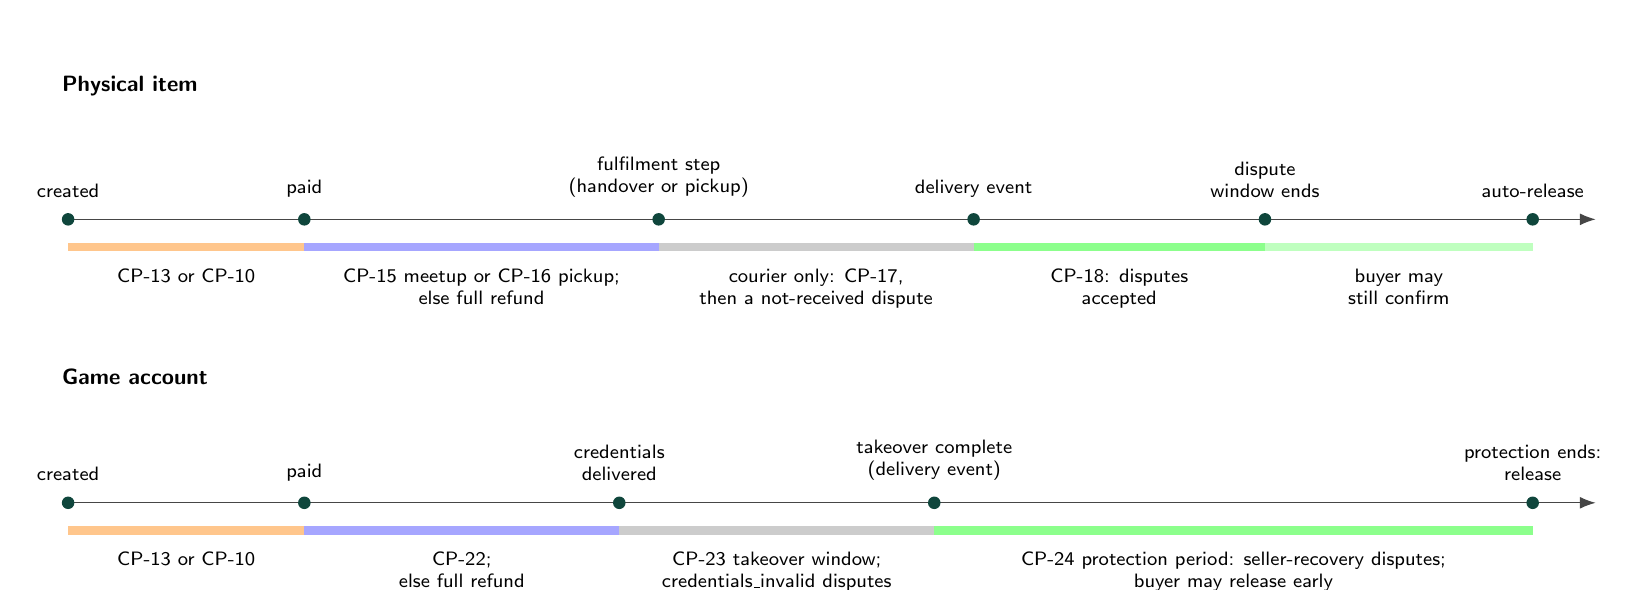
\begin{tikzpicture}[font=\sffamily\scriptsize,
  ev/.style={circle, fill=headcolor, inner sep=1.6pt},
  seg/.style={line width=3pt},
  lb/.style={align=center, font=\sffamily\scriptsize}]
\node[font=\sffamily\footnotesize\bfseries, anchor=west] at (-0.2,1.7) {Physical item};
\draw[-{Latex[length=2mm]}, draw=edge] (0,0) -- (19.4,0);
\foreach \x/\t in {0/created, 3.0/paid, 7.5/fulfilment step\\(handover or pickup), 11.5/delivery event, 15.2/dispute\\window ends, 18.6/auto-release}
  {\node[ev] at (\x,0) {}; \node[lb, above=3pt] at (\x,0.05) {\t};}
\draw[seg, draw=orange!45] (0,-0.35) -- node[below=3pt, lb]{CP-13 or CP-10} (3.0,-0.35);
\draw[seg, draw=blue!35] (3.0,-0.35) -- node[below=3pt, lb]{CP-15 meetup or CP-16 pickup;\\else full refund} (7.5,-0.35);
\draw[seg, draw=gray!40] (7.5,-0.35) -- node[below=3pt, lb]{courier only: CP-17,\\then a not-received dispute} (11.5,-0.35);
\draw[seg, draw=green!45] (11.5,-0.35) -- node[below=3pt, lb]{CP-18: disputes\\accepted} (15.2,-0.35);
\draw[seg, draw=green!25] (15.2,-0.35) -- node[below=3pt, lb]{buyer may\\still confirm} (18.6,-0.35);
\node[font=\sffamily\footnotesize\bfseries, anchor=west] at (-0.2,-2.0) {Game account};
\draw[-{Latex[length=2mm]}, draw=edge] (0,-3.6) -- (19.4,-3.6);
\foreach \x/\t in {0/created, 3.0/paid, 7.0/credentials\\delivered, 11.0/takeover complete\\(delivery event), 18.6/protection ends:\\release}
  {\node[ev] at (\x,-3.6) {}; \node[lb, above=3pt] at (\x,-3.55) {\t};}
\draw[seg, draw=orange!45] (0,-3.95) -- node[below=3pt, lb]{CP-13 or CP-10} (3.0,-3.95);
\draw[seg, draw=blue!35] (3.0,-3.95) -- node[below=3pt, lb]{CP-22;\\else full refund} (7.0,-3.95);
\draw[seg, draw=gray!40] (7.0,-3.95) -- node[below=3pt, lb]{CP-23 takeover window;\\credentials\_invalid disputes} (11.0,-3.95);
\draw[seg, draw=green!45] (11.0,-3.95) -- node[below=3pt, lb]{CP-24 protection period: seller-recovery disputes;\\buyer may release early} (18.6,-3.95);
\end{tikzpicture}}
\caption{Deadlines of an order. Each segment's rule is enforced by a scheduled job (Section~\ref{sec:jobs}) from the times stored on the order and its escrow.}
\label{fig:timeline}
\end{figure}

\begin{itemize}[nosep]
  \item \texttt{payment\_due\_at}: the checkout hold \texttt{CP-13} for fixed-price orders, or the payment window \texttt{CP-10} (or \texttt{CP-11} for a second-chance order) for auctions.
  \item \texttt{fulfilment\_due\_at}, set at payment: \texttt{CP-15} for a meetup handover, \texttt{CP-16} for courier pickup, \texttt{CP-22} for credential delivery. The step to be met is stored in \texttt{fulfilment\_step}.
  \item At the delivery event:
  \begin{itemize}[nosep]
    \item standard orders: \texttt{dispute\_window\_ends\_at} $=$ event $+$ \texttt{CP-18} and \texttt{auto\_release\_at} $=$ event $+$ \texttt{CP-19};
    \item game-account orders (\texttt{game\_protection}): both $=$ event $+$ \texttt{CP-24}, because disputes are accepted throughout the protection period (FR-GAM-16, FR-GAM-17).
  \end{itemize}
  All values come from the parameter version stored on the order, so a later parameter change never alters a running order (FR-OPS-08).
\end{itemize}

\subsection{Fixed-price checkout}
\label{sec:checkout}
\texttt{POST /orders} with listing, quantity, fulfilment method and, for courier, a delivery quote id. One transaction (DC-13):
\begin{enumerate}[nosep]
  \item \texttt{@Verified(buy)} has already passed. Check the order limits CP-27 for buyers verified fewer than 30 days ago (FR-TNS-07), and refuse if the buyer is the seller.
  \item \texttt{ListingsPort.reserve(listing, qty, tx)} runs one conditional update in the Listings schema: decrease available and increase reserved, \emph{only if} the listing is active and available $\ge$ qty. Zero rows updated means ``not available'', returned at once as \texttt{409}. Simultaneous checkouts therefore get definite answers and never over-reserve (FR-FIX-02, FR-FIX-05). Because the update is a single statement, PostgreSQL's row lock serialises concurrent requests without a lost update.
  \item For courier, \texttt{DeliveryPort.getQuote} must return an unexpired quote issued to this buyer for this listing; its fee becomes \texttt{delivery\_fee}. For a game account, the fulfilment is \texttt{game\_account} and the fee is zero.
  \item Insert the order with the listing snapshot, the fee rates (the commission rate depends on \texttt{ProStatus\-Query}) and the parameter version, with \texttt{payment\_due\_at} $=$ now $+$ CP-13. Write \texttt{orders.order.created} to the outbox and audit.
\end{enumerate}

\subsection{Auction and second-chance orders}
\label{sec:auction}
When an auction closes, the Auction unit calls \texttt{OrdersPort.createAuctionOrder} with the winner and price; the payment window is CP-10. The buyer then chooses the fulfilment method (\texttt{PUT /orders/\{id\}/fulfilment}) and pays.

If the window passes unpaid, the scheduled job cancels the order (\texttt{payment\_window\_expired}) and emits \texttt{orders.order.payment\_expired}. The Auction unit then gives the strike and makes the second-chance offer. An accepted offer becomes a \texttt{second\_chance} order with window CP-11. The partial unique index allows only one live order per auction listing, so a second-chance order can exist only after the first is cancelled.

\subsection{Payment}
\label{sec:payment}
\begin{figure}[!htbp]
\centering
\resizebox{\textwidth}{!}{%
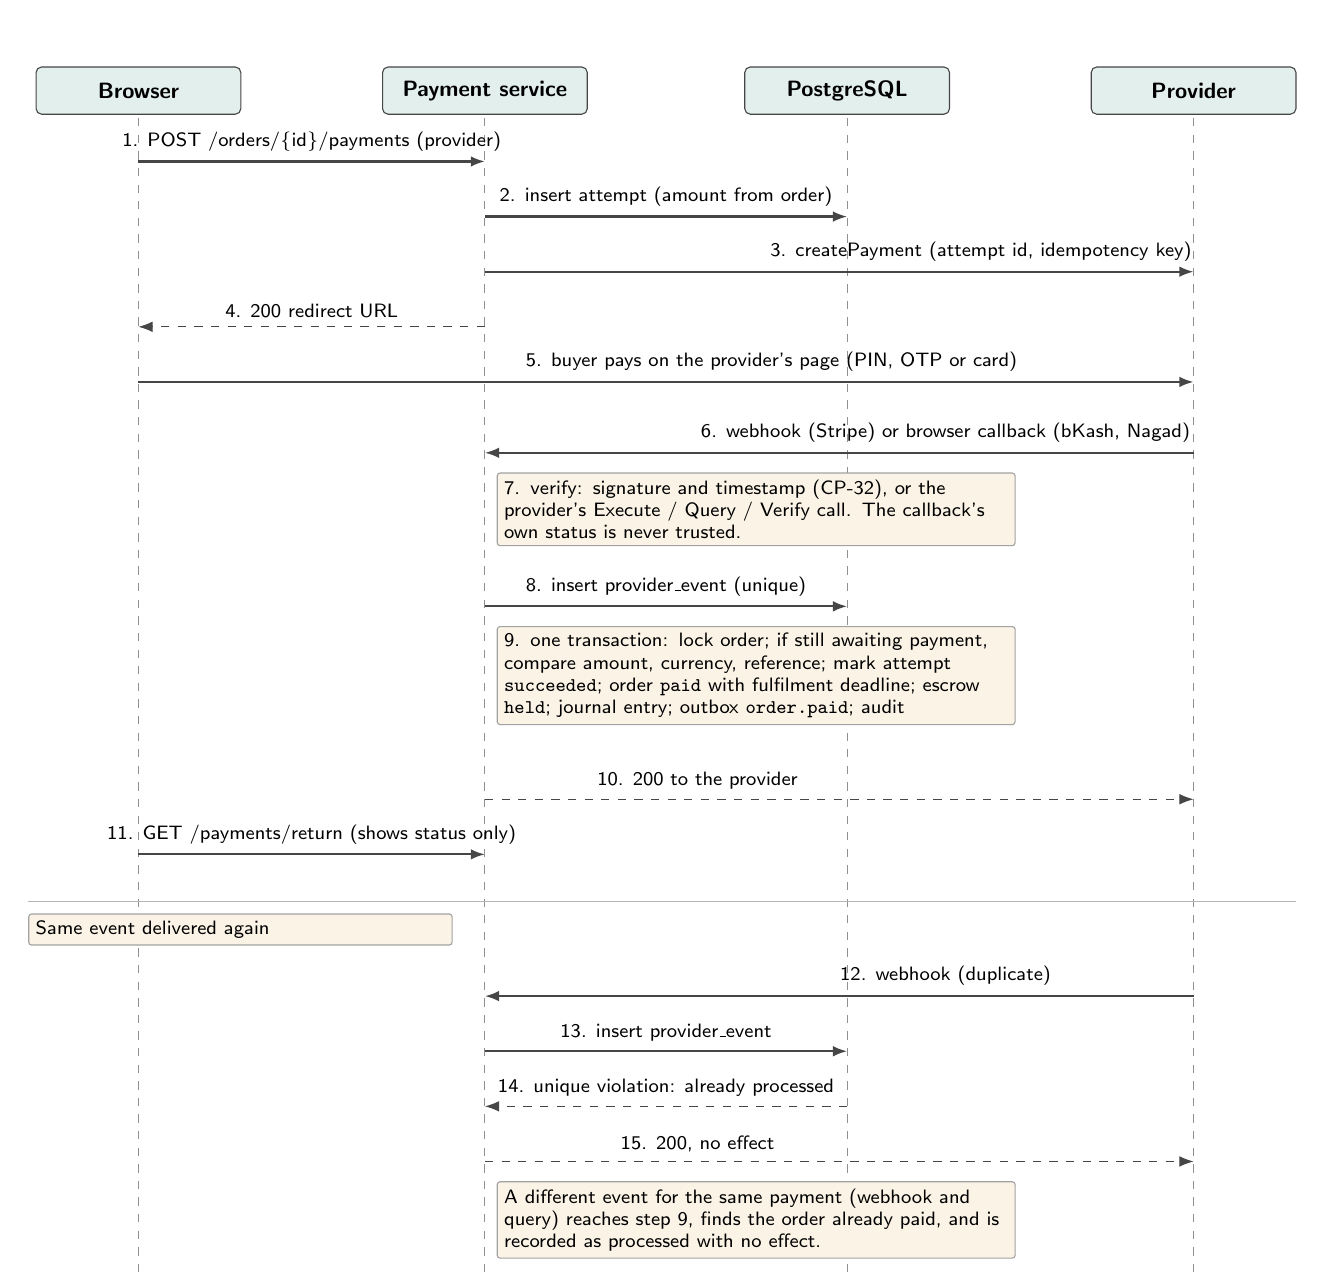
\begin{tikzpicture}[font=\sffamily\scriptsize,
  life/.style={draw=edge!60, dashed},
  hd/.style={draw=edge, fill=boxa, rounded corners=2pt, minimum width=2.6cm, minimum height=0.6cm, font=\sffamily\footnotesize\bfseries},
  msg/.style={-{Latex[length=1.8mm]}, draw=edge, thick},
  ret/.style={-{Latex[length=1.8mm]}, draw=edge, dashed},
  note/.style={draw=edge!50, fill=boxc, align=left, font=\sffamily\scriptsize, inner sep=2.5pt, rounded corners=1pt, text width=6.4cm}]
\def\B{0} \def\O{4.4} \def\D{9.0} \def\V{13.4}
\foreach \x/\n in {\B/Browser, \O/Payment service, \D/PostgreSQL, \V/Provider}{
  \node[hd] at (\x,0) {\n};
  \draw[life] (\x,-0.35) -- (\x,-15.2);}
\draw[msg] (\B,-0.9) -- node[above]{1. POST /orders/\{id\}/payments (provider)} (\O,-0.9);
\draw[msg] (\O,-1.6) -- node[above]{2. insert attempt (amount from order)} (\D,-1.6);
\draw[msg] (\O,-2.3) -- node[above, pos=0.7]{3. createPayment (attempt id, idempotency key)} (\V,-2.3);
\draw[ret] (\O,-3.0) -- node[above]{4. 200 redirect URL} (\B,-3.0);
\draw[msg] (\B,-3.7) -- node[above, pos=0.6]{5. buyer pays on the provider's page (PIN, OTP or card)} (\V,-3.7);
\draw[msg] (\V,-4.6) -- node[above, pos=0.35]{6. webhook (Stripe) or browser callback (bKash, Nagad)} (\O,-4.6);
\node[note, anchor=north west] at (\O+0.15,-4.85) {7. verify: signature and timestamp (CP-32), or the provider's Execute / Query / Verify call. The callback's own status is never trusted.};
\draw[msg] (\O,-6.55) -- node[above]{8. insert provider\_event (unique)} (\D,-6.55);
\node[note, anchor=north west] at (\O+0.15,-6.8) {9. one transaction: lock order; if still awaiting payment, compare amount, currency, reference; mark attempt \texttt{succeeded}; order \texttt{paid} with fulfilment deadline; escrow \texttt{held}; journal entry; outbox \texttt{order.paid}; audit};
\draw[ret] (\O,-9.0) -- node[above, pos=0.3]{10. 200 to the provider} (\V,-9.0);
\draw[msg] (\B,-9.7) -- node[above]{11. GET /payments/return (shows status only)} (\O,-9.7);
\draw[draw=edge!40] (-1.4,-10.3) -- (14.7,-10.3);
\node[note, anchor=north west, text width=5.2cm] at (-1.4,-10.45) {Same event delivered again};
\draw[msg] (\V,-11.5) -- node[above, pos=0.35]{12. webhook (duplicate)} (\O,-11.5);
\draw[msg] (\O,-12.2) -- node[above]{13. insert provider\_event} (\D,-12.2);
\draw[ret] (\D,-12.9) -- node[above]{14. unique violation: already processed} (\O,-12.9);
\draw[ret] (\O,-13.6) -- node[above, pos=0.3]{15. 200, no effect} (\V,-13.6);
\node[note, anchor=north west] at (\O+0.15,-13.85) {A different event for the same payment (webhook and query) reaches step 9, finds the order already paid, and is recorded as processed with no effect.};
\end{tikzpicture}}
\caption{Payment confirmation and a duplicate delivery of the same event (FR-PAY-02 to FR-PAY-05).}
\label{fig:seq-pay}
\end{figure}

\begin{itemize}[nosep]
  \item \textbf{Start.} Payment can start only while the order is \texttt{awaiting\_payment} with a fulfilment method. The game-account unit must report the order ready: the disclosure acknowledged and the buyer's public key present. The attempt's amount is the order total. Starting a payment inside the hold extends \texttt{payment\_due\_at} once, to the attempt's expiry (DV-11), so that a buyer who is part-way through the provider's page is not cancelled under them.
  \item \textbf{Mismatch} (FR-PAY-03). If the verified amount, currency or reference differs, the attempt becomes \texttt{succeeded\_rejected}. A full refund is created and an \texttt{amount\_mismatch} issue raised; the order stays unpaid.
  \item \textbf{Late payment.} If the order was already cancelled when a genuine success arrives, the payment is \texttt{succeeded\_rejected}, refunded in full and raised as \texttt{late\_payment}. The expiry job queries in-flight attempts before cancelling, which makes this rare.
  \item \textbf{Duplicate payment.} If the order is already paid by another attempt, the second one is \texttt{succeeded\_duplicate} and refunded in full.
  \item \textbf{Failure.} A failed or abandoned attempt leaves the order awaiting payment, and the buyer may try again until \texttt{payment\_due\_at}. Provider calls are retried with exponential backoff and jitter using the same idempotency key (FR-PAY-16).
\end{itemize}

\subsection{Fulfilment steps and the delivery event}
\label{sec:steps}
Delivery and Game-Account report progress through \texttt{EscrowCommands}, inside their own transactions (DC-13):
\begin{itemize}[nosep]
  \item \texttt{recordFulfilmentStep} sets \texttt{fulfilment\_done\_at}. The steps are courier pickup and credential delivery. A meetup handover counts both as the step and as the delivery event.
  \item \texttt{recordDeliveryEvent} sets the event time and source (handover code, courier \texttt{delivered}, takeover complete) and the escrow's dispute-window and auto-release times. It writes \texttt{orders.order.delivered}.
  \item \texttt{refundCourierReturned} refunds the buyer in full, including the fee. Any courier charge is posted as \texttt{expense\_courier\_returns} (FR-DLV-12).
\end{itemize}
A step or event that arrives twice, or for an order in the wrong state, is ignored and logged. The first recorded time stands.

\subsection{Release}
\label{sec:release}
Release happens by buyer confirmation after the delivery event (\texttt{confirm-receipt}); by the auto-release job at \texttt{auto\_release\_at} with no dispute open; or, for game accounts, by early release with step-up. Each runs one transaction:
\begin{enumerate}[nosep]
  \item lock the order and then the escrow (fixed lock order) and re-check the state;
  \item compute the split with \texttt{item\_refund} $=$ 0;
  \item set the escrow to \texttt{released} and write the history row;
  \item insert the settlement record and post the release entry;
  \item create the payout, choosing its status:
  \begin{itemize}[nosep]
    \item \texttt{held} if the seller is suspended for fraud;
    \item \texttt{waiting\_account} if there is no payout account;
    \item \texttt{waiting\_cooling\_off} until the account is effective;
    \item otherwise \texttt{pending};
  \end{itemize}
  \item close the order, write \texttt{orders.escrow.released} to the outbox, and audit.
\end{enumerate}
Because confirm-receipt, the release job, a dispute being opened and a cancellation all take the same escrow row lock, they are serialised. Whichever commits first decides, and the others find the new state and stop. Physical disputes close CP-19 $-$ CP-18 (two days by default) before auto-release, so the two never compete. For game accounts both end at the same moment, and a dispute is accepted only strictly before \texttt{auto\_release\_at}.

\subsection{Cancellation and deadline refunds}
\label{sec:cancel}
\begin{itemize}[nosep]
  \item \textbf{Before payment.} The expiry job cancels unpaid orders after \texttt{payment\_due\_at} (\texttt{checkout\_expired} or \texttt{payment\_window\_expired}). Before cancelling, it queries any in-flight attempt, so a payment that succeeded without a callback is confirmed rather than lost. Listings returns the reserved stock on \texttt{order.cancelled} (FR-FIX-03).
  \item \textbf{After payment, before the delivery event} (FR-PAY-09). The buyer requests cancellation and the seller accepts, or the seller cancels unilaterally. Either way the escrow becomes \texttt{refunded} for the full amount. A unilateral cancellation also emits \texttt{orders.order.cancelled\_by\_seller} for the strike.
  \item \textbf{Missed fulfilment deadline} (FR-PAY-08). The fulfilment job refunds every paid order whose required step is not recorded by \texttt{fulfilment\_due\_at} and that has no open dispute.
  \item \textbf{Stalled courier delivery.} If the item was picked up but no delivery event follows within CP-17 $+$ CP-18, and no dispute is opened, the job raises a \texttt{stalled\_delivery} issue for an operator rather than releasing or refunding automatically (DV-12).
\end{itemize}

\subsection{Refunds}
\label{sec:refunds}
A refund row is created, with its own idempotency key, in the same transaction as the decision that causes it, together with its ledger entry. The refund worker then calls the provider's refund function on the original payment:
\begin{itemize}[nosep]
  \item success moves the refund to \texttt{succeeded} and posts the ``refund paid out'' entry;
  \item a failure is retried with backoff up to DV-13;
  \item after the retries are exhausted, or when the provider cannot refund (\texttt{unsupported}), the refund becomes \texttt{manual\_required}, an operator issue is raised and the buyer is told when to expect the money (FR-PAY-12).
\end{itemize}
The database trigger guarantees that the refunds of one payment never add up to more than it.

\subsection{Disputes}
\label{sec:disputes}
The Disputes unit calls \texttt{freezeForDispute}, accepted only if \texttt{EscrowQuery.disputeAllowed}: the escrow is \texttt{held} and the time is inside the window (FR-DSP-01, FR-DSP-11). This moves the escrow to \texttt{frozen\_disputed}, which stops every automatic release (FR-DSP-02). \texttt{applyDisputeOutcome} executes the decision (FR-DSP-06):
\begin{itemize}[nosep]
  \item \textbf{release} works as Section~\ref{sec:release};
  \item \textbf{full refund} refunds the whole item price, and the delivery fee too if the courier never picked up. If the courier did pick up, the fee stays with the courier and platform, so the escrow ends \texttt{partially\_refunded} even though the buyer received everything refundable;
  \item \textbf{partial} applies the split with the decided item refund;
  \item \textbf{refund after return} leaves the escrow frozen until the Disputes unit reports the item back. A return fare paid by the buyer is deducted from the refund; one paid by the seller becomes a \texttt{seller\_receivable}, recovered from later payouts.
\end{itemize}
\texttt{withdrawDispute} returns the escrow to \texttt{held} with \texttt{auto\_release\_at} $=$ the later of the original time and now $+$ 24 hours (FR-DSP-10). Decisions requiring four-eyes approval (CP-30) are approved in the Disputes unit before this call.

\subsection{Payout accounts and payouts}
\label{sec:payouts}
\begin{itemize}[nosep]
  \item \textbf{Wallet.} An MFS wallet is accepted only if its number equals the seller's verified mobile number, from \texttt{IdentityQuery.getVerifiedPhone}. It enters \texttt{cooling\_off} with \texttt{effective\_at} $=$ now $+$ CP-29 (FR-PAY-17, FR-PAY-18).
  \item \textbf{Bank account.} A bank account enters \texttt{pending\_review}. An operator compares the account name with the KYC name; reading that name through \texttt{getKycLegalName} is audited. Only after approval does the account go into cooling-off.
  \item \textbf{Change.} Adding or changing an account requires step-up and emits \texttt{payments.\allowbreak payout\_account.\allowbreak changed}, so the seller's number and e-mail are alerted. The previous account becomes \texttt{replaced}. Payouts waiting for cooling-off are sent once the new account is effective.
  \item \textbf{Sending.} The payout worker sends \texttt{pending} payouts through the payout adapter with the payout's idempotency key, then posts the ``payout sent'' entry. Failures are retried and then raised as \texttt{payout\_failed}.
  \item \textbf{Fraud hold.} When Unit~1 reports a suspension for fraud, the seller's pending payouts become \texttt{held} and new ones are created \texttt{held} (FR-TNS-05), until an operator lifts the hold.
\end{itemize}

\subsection{Reconciliation and chargebacks}
\label{sec:recon}
\begin{itemize}[nosep]
  \item \textbf{Every CP-46} (FR-PAY-15), the reconciliation job:
  \begin{itemize}[nosep]
    \item queries attempts that have been in flight longer than DV-15;
    \item queries refunds sent but not confirmed;
    \item checks paid orders whose attempt lacks a provider transaction id.
  \end{itemize}
  Each query result is recorded as a provider event with a derived id, such as \texttt{query:\allowbreak\{attempt\}:\allowbreak\{status\}}, and processed through the normal idempotent path. A result that contradicts the ledger raises a \texttt{provider\_disagrees} issue instead of being applied.
  \item \textbf{Daily}, where the provider offers a settlement report, the job compares the day's totals with \texttt{provider\_clearing} postings.
  \item \textbf{Chargebacks} (FR-PAY-20, Could). A Stripe dispute event records a chargeback and posts it to \texttt{seller\_receivable}. Later payouts to that seller are reduced until it is recovered, and an operator is notified.
\end{itemize}

\subsection{Monetization}
\label{sec:mon}
\begin{itemize}[nosep]
  \item \textbf{Commission and delivery margin} are taken in the split from the rates stored on the order (FR-MON-01 to FR-MON-03, FR-MON-10). There is no listing fee and no per-click charge (FR-MON-04).
  \item \textbf{Featured listing} (Could). The seller pays the CP-37 fee through a \texttt{featured\_listing} attempt. On confirmation the purchase starts and \texttt{payments.featured.started} tells Listings to show the label; a job ends it on time.
  \item \textbf{Pro Seller} (Could). Card subscriptions use Stripe's recurring billing, confirmed by webhook. Because MFS wallets do not support recurring charges, MFS subscribers pay each month through a \texttt{subscription} attempt after a reminder. Two failed or missed renewals move the subscription to \texttt{lapsed} (FR-MON-08). \texttt{ProStatusQuery.isPro} is read when an order is created, so the rate applies only to orders created while the subscription is active.
\end{itemize}

\subsection{Scheduled jobs}
\label{sec:jobs}
Each job selects due rows with \texttt{FOR UPDATE SKIP LOCKED} in batches, re-checks the row's state inside its transaction, and acts on the recorded deadline times. A job can therefore run on several instances at once, can be re-run safely, and catches up after downtime without acting twice (NFR-REL-03).
\begin{dtable}{@{}>{\raggedright\arraybackslash}p{3.6cm}>{\raggedright\arraybackslash}p{1.8cm}>{\raggedright\arraybackslash}p{9.8cm}@{}}
\toprule
\textbf{Job} & \textbf{Every} & \textbf{Action} \\ \midrule \endhead
Payment expiry & 1 min & Query in-flight attempts; then cancel orders past \texttt{payment\_due\_at}. \\
Fulfilment deadline & 1 min & Refund paid orders whose fulfilment step is overdue (FR-PAY-08). \\
Auto-release & 1 min & Release held escrows past \texttt{auto\_release\_at} (FR-PAY-07b, FR-GAM-17). \\
Stalled delivery & 1 hour & Raise \texttt{stalled\_delivery} issues (DV-12). \\
Reconciliation & CP-46 & As above (FR-PAY-15). \\
Refund worker & 30 s & Send pending refunds; retry; mark \texttt{manual\_required} (FR-PAY-12). \\
Payout worker & 1 min & Send payouts that are due; release cooled-off ones (FR-PAY-19). \\
Cancellation lapse & 1 hour & Lapse pending requests at the delivery event or the fulfilment deadline. \\
Monetization & 5 min & End featured periods; process renewals and lapses. \\
Outbox & 5 s & Publish pending events. \\
\bottomrule
\end{dtable}
\section{Security Design}

\subsection{Verifying provider messages}
\label{sec:verify}
\begin{itemize}[nosep]
  \item \textbf{Stripe webhooks.} The raw request body is verified against the \texttt{Stripe-Signature} header with the webhook secret of the current environment; the signed timestamp must be within CP-32. The event id is stored in \texttt{provider\_events} before processing, so a replay is a unique violation and has no effect (SEC-PAY-03, SEC-PAY-04).
  \item \textbf{bKash and Nagad callbacks.} These arrive through the buyer's browser and are untrusted. The callback URL contains the attempt id and an HMAC of it (``signed state''), which stops a forged callback from naming another attempt. In any case the server never acts on the callback's content: it calls the provider's execute, query or verify API with its own credentials and acts only on that answer.
  \item \textbf{Every confirmation}, whatever its route, must match the attempt: amount, currency BDT and merchant reference (FR-PAY-03). The amount is computed on the server; any amount from the client is ignored (SEC-PAY-06).
\end{itemize}

\subsection{Card and wallet data}
Card numbers are entered only on Stripe's hosted Checkout page, reached by redirect, so TrustBazaar's pages contain no card form and no payment script. This keeps the platform within SAQ A (SEC-PAY-01, NFR-CMP-03). MFS PINs and OTPs are entered only on bKash's or Nagad's pages (SEC-PAY-02). The database stores only provider ids and references, and the last four digits of a bank account; the full bank account number is encrypted with Unit~1's field key.

\subsection{Credentials, environments and idempotency}
\begin{itemize}[nosep]
  \item Provider credentials are read from environment variables. At start-up the backend checks that every credential matches the configured mode, and refuses to start on a mismatch (SEC-PAY-05). For example, Stripe keys must begin \texttt{sk\_test\_} in sandbox mode and \texttt{sk\_live\_} only in production.
  \item Every attempt, refund and payout has its own idempotency key, stored before the provider is called, and sent as Stripe's \texttt{Idempotency-Key} header or as the merchant invoice or order number for bKash and Nagad (SEC-PAY-07). A retry after a timeout therefore cannot create a second charge, refund or payout. Before retrying a bKash or Nagad refund whose outcome is unknown, the worker queries the provider first.
\end{itemize}

\subsection{Abuse and fraud controls}
\begin{itemize}[nosep]
  \item Order limits CP-27 for newly verified buyers (FR-TNS-07); checkout and payment start are rate-limited (SEC-ABU-01).
  \item Payouts go only to a wallet on the seller's own verified number, or to a bank account in the seller's KYC name. A changed account waits CP-29 before receiving money, and both contact channels are alerted. These defeat the common pattern of taking over an account and redirecting its payouts.
  \item Fraud holds stop payouts while Trust \& Safety investigates (FR-TNS-05).
  \item Release before the delivery event is impossible. Scammers often press buyers to ``confirm now'', and the system cannot do so.
\end{itemize}

\subsection{Operators}
Operators can resolve reconciliation issues, approve bank accounts and lift payout holds, each with a recorded reason and an audit entry. They cannot move money in any other way: there is no endpoint to edit an order, an escrow or a ledger entry, and the database refuses such edits from the application role (SRS C-5, FR-OPS-02).

% ------------------------------------------------------------------
\section{Parameters}
\textbf{SRS parameters used:} CP-10, CP-11 (payment windows); CP-13 (checkout hold); CP-15, CP-16, CP-17 (fulfilment deadlines); CP-18, CP-19 (dispute window, auto-release); CP-22, CP-24 (game account); CP-25, CP-26 (fees); CP-27 (order limits); CP-29 (payout cooling-off); CP-30 (four-eyes, applied in Disputes); CP-32 (webhook tolerance and event retention); CP-37 (featured fees); CP-46 (reconciliation interval).

\textbf{Design values introduced} (proposed for the SRS parameter table, continuing Unit~1's DV-1 to DV-10):
\begin{dtable}{@{}>{\bfseries}p{1.3cm}>{\raggedright\arraybackslash}p{6.0cm}>{\raggedright\arraybackslash}p{3.0cm}>{\raggedright\arraybackslash}p{4.9cm}@{}}
\toprule
\textnormal{\textbf{ID}} & \textbf{Value} & \textbf{Default} & \textbf{Reason} \\ \midrule \endhead
DV-11 & Payment attempt lifetime (and hold extension) & 15 minutes & Time on the provider's page; extends the hold once. \\
DV-12 & Stalled courier delivery review & CP-17 $+$ CP-18 after pickup & Hands the case to a person rather than guessing. \\
DV-13 & Refund retries before manual handling & 8 attempts over 24 hours & Rides out provider outages. \\
DV-14 & Payout retries before raising an issue & 6 attempts over 12 hours & As above. \\
DV-15 & In-flight attempt age before reconciliation queries it & 2 minutes & Most callbacks arrive within seconds. \\
DV-16 & Cancellation request lapse & At the delivery event or fulfilment deadline & No request outlives the order's next step. \\
\bottomrule
\end{dtable}

% ------------------------------------------------------------------
\section{Testing}
\begin{dtable}{@{}>{\raggedright\arraybackslash}p{3.2cm}>{\raggedright\arraybackslash}p{12cm}@{}}
\toprule
\textbf{Level} & \textbf{Cases} \\ \midrule \endhead
Database (done) & 45 checks in \texttt{02\_orders\_payments\_tests.sql}. Each rejection is required to name the intended constraint, so no check can pass because a different rule fired. They include the SRS worked example, its partial-refund variant and 20{,}000 random splits. A concurrency test sends 15 simultaneous confirmations of one payment and produces exactly one escrow (Appendix~\ref{app:tests}). \\
Unit & \texttt{SettlementService} against \texttt{payments.split()} on random inputs (identical results); deadline arithmetic from stored parameter versions; each adapter's \texttt{verify} rejects a bad signature, a stale timestamp and a mismatched amount; the payout-status choice. \\
Integration & 50 simultaneous checkouts for the last unit, with a Listings stub, give exactly one reservation (AC-2). Confirm-receipt racing auto-release and dispute opening gives exactly one outcome. Expiry with an in-flight attempt confirms rather than cancels. A late payment is refunded; a duplicate payment is refunded. A refund retried after a timeout does not refund twice. The outbox survives a crash between commit and publication. \\
Sandbox contract & For each provider in its sandbox: pay, cancel on the provider page, refund, partial refund, replayed webhook, forged callback. \\
Acceptance & AC-2, AC-3, AC-4 and AC-6 (SRS Appendix~A), each automated under the reference load (NFR-PERF-08). \\
\bottomrule
\end{dtable}

% ------------------------------------------------------------------
\section{Notes for Integration}
\label{sec:notes}
\begin{enumerate}[label=\textbf{I-\arabic*}, leftmargin=*, nosep]
  \setcounter{enumi}{7}
  \item \textbf{Unit 1 port addition.} \texttt{IdentityQuery.getPrincipal} should also return \texttt{verifiedAt} for the CP-27 limits, and Unit~1 should emit a fraud flag with \texttt{identity.account.suspended} so that payouts can be held.
  \item \textbf{Listings (Unit 3)} must provide \texttt{reserve} and \texttt{release} as single conditional updates (DC-13), mark units sold on \texttt{order.paid} and release them on \texttt{order.cancelled}.
  \item \textbf{Delivery (Unit 4)} issues quotes bound to buyer, listing and expiry, and reports pickup, handover code, delivered and returned through \texttt{EscrowCommands}.
  \item \textbf{Game-Account (Unit 5)} reports credential delivery and takeover completion, and exposes \texttt{assertCheckoutReady}.
  \item \textbf{Disputes (Unit 7)} owns dispute windows by type, four-eyes approval of large outcomes, and the return shipment for ``refund after return''.
  \item \textbf{SRS clarifications proposed:}
  \begin{itemize}[nosep]
    \item a ``full refund'' outcome after courier pickup ends \texttt{partially\_refunded}, because the delivery fee is not refundable;
    \item add DV-11 to DV-16 to the SRS parameter table;
    \item MFS subscriptions renew by monthly payment, not automatic charge.
  \end{itemize}
\end{enumerate}

% ------------------------------------------------------------------
\appendix
\section{Traceability}
\label{app:trace}
{\small\begin{longtable}{@{}>{\ttfamily}p{2.4cm}>{\raggedright\arraybackslash}p{10.6cm}>{\raggedright\arraybackslash}p{2.2cm}@{}}
\toprule \textnormal{\textbf{Requirement}} & \textbf{Design element} & \textbf{Section} \\ \midrule \endhead
FR-PAY-01 & Three adapters behind one interface; sandbox and test modes & \ref{sec:adapters} \\
FR-PAY-02 & Confirmation only from webhook signature or provider query; return page shows status only & \ref{sec:payment}, \ref{sec:verify} \\
FR-PAY-03 & Amount, currency and reference compared; mismatch gives \texttt{succeeded\_rejected} and a refund & \ref{sec:payment} \\
FR-PAY-04 & Unique provider events; one successful attempt per order; concurrency test & \ref{sec:payment}, \ref{sec:data} \\
FR-PAY-05 & Escrow row created \texttt{held} with the full amount & \ref{sec:payment} \\
FR-PAY-06 & \texttt{escrow\_transition} trigger; Figure~\ref{fig:states} & \ref{sec:data} \\
FR-PAY-07 & Release paths and shared escrow lock; no confirm before the delivery event & \ref{sec:release} \\
FR-PAY-08 & Fulfilment step and deadline columns; fulfilment job & \ref{sec:deadlines}, \ref{sec:cancel} \\
FR-PAY-09 & Cancellation requests; seller cancellation with strike event & \ref{sec:cancel} \\
FR-PAY-10 & \texttt{escrow\_history}, append-only & \ref{sec:data} \\
FR-PAY-11 & \texttt{payments.split()}; item refund first; commission on released part & \ref{sec:split} \\
FR-PAY-12 & Refund rows, worker, retries, \texttt{manual\_required} & \ref{sec:refunds} \\
FR-PAY-13 & \texttt{payments.settlements} written with the terminal transition & \ref{sec:ledger} \\
FR-PAY-14 & bigint poisha; half-up rounding; sums checked by constraint; 20{,}000-case property test & \ref{sec:split} \\
FR-PAY-15 & Reconciliation job and issues queue & \ref{sec:recon} \\
FR-PAY-16 & Backoff with jitter reusing idempotency keys & \ref{sec:payment} \\
FR-PAY-17 & Wallet equals verified number; bank name check by operator & \ref{sec:payouts} \\
FR-PAY-18 & Step-up; alert event; cooling-off \texttt{effective\_at} & \ref{sec:payouts} \\
FR-PAY-19 & Payouts table and worker; simulated adapter & \ref{sec:payouts} \\
FR-PAY-20 & Chargebacks posted to \texttt{seller\_receivable} & \ref{sec:recon} \\
FR-PAY-21 & Receipt and statement endpoints from settlements & \ref{sec:api} \\
FR-FIX-01 & Verified(buy); buyer $\neq$ seller constraint & \ref{sec:checkout} \\
FR-FIX-02 & \texttt{ListingsPort.reserve} in the order transaction (DC-13) & \ref{sec:checkout} \\
FR-FIX-03 & Payment expiry job; \texttt{order.cancelled} returns stock & \ref{sec:cancel} \\
FR-FIX-04 & \texttt{order.paid} lets Listings mark units sold & \ref{sec:checkout} \\
FR-FIX-05 & Single conditional update gives a definite answer per request & \ref{sec:checkout} \\
FR-AUC-14 & \texttt{OrdersPort.createAuctionOrder}; window CP-10; one live order per auction & \ref{sec:auction} \\
FR-AUC-15 & Expiry emits \texttt{payment\_expired}; second-chance orders with CP-11 & \ref{sec:auction} \\
FR-DLV-11 & Pickup deadline CP-16; stalled-delivery review & \ref{sec:cancel} \\
FR-DLV-12 & \texttt{refundCourierReturned}; courier return expense & \ref{sec:steps} \\
FR-DLV-13 & Margin and courier payout in the split & \ref{sec:split} \\
FR-GAM-10 & Credential delivery deadline CP-22 refunds & \ref{sec:deadlines}, \ref{sec:cancel} \\
FR-GAM-17 & \texttt{game\_protection} policy; early release with step-up & \ref{sec:deadlines}, \ref{sec:release} \\
FR-DSP-02 & \texttt{freezeForDispute}; frozen escrow names its dispute & \ref{sec:disputes} \\
FR-DSP-06 & \texttt{applyDisputeOutcome}: release, full, partial, after return & \ref{sec:disputes} \\
FR-DSP-10 & \texttt{withdrawDispute} with the later of the two release times & \ref{sec:disputes} \\
FR-DSP-11 & \texttt{disputeAllowed} requires \texttt{held} and the window & \ref{sec:disputes} \\
FR-MON-01 & Commission in the split from the rate stored on the order & \ref{sec:split}, \ref{sec:mon} \\
FR-MON-02 & \texttt{ProStatusQuery} read at order creation & \ref{sec:mon} \\
FR-MON-03 & Delivery margin in the split & \ref{sec:split} \\
FR-MON-04 & No listing or click fees exist in the design & \ref{sec:mon} \\
FR-MON-05 & Featured purchases through attempts; started and ended events & \ref{sec:mon} \\
FR-MON-06 & Subscriptions table; Stripe recurring, MFS monthly & \ref{sec:mon} \\
FR-MON-07 & Subscription payments confirmed like purchases & \ref{sec:mon} \\
FR-MON-08 & Lapse after failed renewals; event to Listings & \ref{sec:mon} \\
FR-MON-09 & \texttt{payments.revenue\_log} view & \ref{sec:ledger} \\
FR-MON-10 & Rates and parameter version stored on the order & \ref{sec:checkout} \\
FR-TNS-05 & Payout holds on fraud suspension & \ref{sec:payouts} \\
FR-TNS-07 & CP-27 checked at checkout & \ref{sec:checkout} \\
FR-ACC-11 & \texttt{AccountClosureCheck} implemented by this unit & \ref{sec:api} \\
SEC-PAY-01 & Stripe Checkout by redirect: SAQ A & \ref{sec:verify} \\
SEC-PAY-02 & PINs and OTPs only on provider pages; references only & \ref{sec:verify} \\
SEC-PAY-03 & Signature check, or the provider's own query & \ref{sec:verify} \\
SEC-PAY-04 & Timestamp tolerance; unique provider events & \ref{sec:verify} \\
SEC-PAY-05 & Start-up check of credential mode & \ref{sec:verify} \\
SEC-PAY-06 & Server-computed amounts; client amounts ignored & \ref{sec:verify} \\
SEC-PAY-07 & Idempotency keys on attempts, refunds, payouts & \ref{sec:verify} \\
IF-SW-01 & bKash adapter & \ref{sec:adapters} \\
IF-SW-02 & Nagad adapter & \ref{sec:adapters} \\
IF-SW-03 & Stripe adapter & \ref{sec:adapters} \\
IF-UI-04 & Checkout endpoint returns full price breakdown & \ref{sec:api} \\
IF-UI-05 & Order view with escrow state and deadlines & \ref{sec:api}, \ref{sec:deadlines} \\
IF-UI-08 & Payout account, payouts, statements endpoints & \ref{sec:api} \\
NFR-PERF-06 & Confirmation in one transaction after verification & \ref{sec:payment} \\
NFR-PERF-08 & Database barriers hold under concurrency (tests) & \ref{app:tests} \\
NFR-REL-02 & Acknowledge only after commit & \ref{sec:payment} \\
NFR-REL-03 & Jobs with SKIP LOCKED acting on stored times & \ref{sec:jobs} \\
NFR-REL-04 & Hold extension; outage handling through expiry queries & \ref{sec:payment} \\
NFR-CMP-02 & Ledger maps to a licensed provider in production & \ref{sec:ledger} \\
NFR-CMP-03 & SAQ A scope & \ref{sec:verify} \\
NFR-CMP-05 & Payouts marked simulated; sandbox modes & \ref{sec:adapters} \\
DR-03 & \texttt{listing\_snapshot} on every order & \ref{sec:data} \\
DR-05 & Orders, escrow history, settlements, refunds, payouts, provider references, events & \ref{sec:data} \\
DR-10 & Append-only histories and balanced ledger & \ref{sec:data} \\
SEC-LOG-01 & Every money action audited in its transaction (DC-8); escrow history & \ref{sec:release}, \ref{sec:data} \\
\bottomrule\end{longtable}}


\section{Database Schema and Tests}
\label{app:ddl}
\subsection{Test results}
\label{app:tests}
Loaded after the Unit~1 schema in PostgreSQL 16, using PostgreSQL 15 features only. Every check passed. The concurrency test is listed after the script output.
{\scriptsize
\begin{verbatim}
PASS  FR-FIX-01 buyer cannot buy own listing [buyer_not_seller]
PASS  total must equal item price plus delivery fee [total_matches]
PASS  FR-LST-05 auction order has quantity 1 [auction_single_unit]
PASS  FR-DLV-02 self-pickup adds no delivery fee [fee_only_for_courier]
PASS  FR-GAM-06 a game account cannot go by courier [game_fulfilment_matches]
PASS  an order cannot be paid before a fulfilment method is chosen [paid_needs_fulfilment]
PASS  a paid order must carry its fulfilment deadline (FR-PAY-08) [paid_needs_deadline]
PASS  FR-AUC-14 one live order per auction [orders_one_live_auction]
PASS  FR-AUC-15 second-chance order allowed after the winner's order is cancelled
PASS  AC-4 an order can be paid only once [attempts_one_success_per_order]
PASS  a second successful payment is recorded as a duplicate (to be refunded)
PASS  only BDT is accepted [attempts_currency_check]
PASS  SEC-PAY-04 a replayed provider event is rejected [provider_events_provider_event_id_key]
PASS  FR-PAY-05 escrow must start in held [must start in held]
PASS  FR-PAY-06 held -> partially_refunded is not a permitted transition [is not permitted]
PASS  FR-DSP-02 a frozen escrow names its dispute [escrow_frozen_has_dispute]
PASS  amount collected cannot change [amount_collected is fixed]
PASS  a delivery event needs the fulfilment step first [delivery_after_fulfilment]
PASS  dispute window must end before auto-release [escrow_window_before_release]
PASS  a partial refund must leave something released [escrow_partial_both]
PASS  a terminal escrow cannot change again [is not permitted]
PASS  FR-PAY-10 escrow history is append-only [append-only]
PASS  SRS worked example, release: 500 + 15 + 135 + 9,500 = 10,150 BDT
PASS  SRS worked example, partial refund of BDT 2,000: commission 400, seller 7,600
PASS  courier never picked up: the whole delivery fee is refunded
PASS  half-up rounding to the poisha: 5% of 33 poisha is 2 (1.65 rounds up)
PASS  FR-PAY-14 property: 20,000 random cases always add up exactly and never go negative
PASS  item refund larger than the item price is refused [out of range]
PASS  FR-PAY-13 one settlement record per order, never rewritten [append-only]
PASS  FR-PAY-14 a settlement whose parts do not add up is refused [settlement_parts_sum]
PASS  refunds can never exceed the payment [exceed payment]
PASS  an unbalanced journal entry is refused at commit [does not balance]
PASS  balanced entries are accepted
PASS  escrow liability of a settled order nets to zero
PASS  FR-MON-09 revenue log shows commission 400 and margin 15 BDT
PASS  ledger balance equals settlement record
PASS  journal lines are append-only [append-only]
PASS  FR-PAY-17 one current payout account per seller [payout_account_one_current]
PASS  FR-PAY-17 a bank account becomes usable only after an operator check [bank_reviewed]
PASS  one payout per order [payouts_order_id_key]
PASS  FR-TNS-05 a held payout records why [payout_hold_reason]
PASS  outbox events belong to this unit [outbox_event_type_check]
PASS  application role cannot rewrite escrow history [permission denied]
PASS  application role cannot change the ledger chart of accounts [permission denied]
PASS  application role cannot delete orders [permission denied]

Concurrency test: 15 simultaneous confirmations of one payment
(10 deliveries of the same webhook event + 5 different confirmation events):
  escrows created = 1, successful attempts = 1, provider events recorded = 1, order status = paid
\end{verbatim}
}

\subsection{Schema}
\lstinputlisting[language=SQLpg]{sql/02_orders_payments.sql}
\end{document}
